%\subsection{Motivation: spatial locality} 
% KV-stores are everywhere
Key-value stores (KV-stores) are widely used nowadays by a broad range of applications. As the 
``driving factors'' of the NoSQL market, which is expected to garner \$4.2B by 2020~\cite{alliedmarketresearch}, they are projected
to continue to increase in popularity.

% In many applications, keys are composite
KV-stores provide a simple programming model. 
Data is an ordered collection of key-values pairs, and  the API supports random writes, 
random reads, and range queries. 

A common design pattern is the use of \emph{composite} 
keys that represent an agglomerate of attributes.
%, where the attribute that is most important for range query performance is the key prefix. 
This approach arises in many domains, for example: 
(1) Mobile analytics services such as Flurry Analytics~\cite{flurry} aggregate statistics 
on data identified by composite keys consisting of attributes such as app id, device, time, location, 
event id, etc. The query API~\cite{flurry-api} is app id-centric, hence this dimension is the key prefix.
(2) In messaging and email, keys are typically a concatenation of user id with additional dimensions 
such as thread id, time, and post id. A query in Facebook Messenger may retrieve, e.g., the last 100 messages for a 
given user~\cite{Borthakur:2011:AHG:1989323.1989438}. %, or the hourly impression counts %over the last 24 hours for a given advertiser. 
(3) In Facebook's social network, a graph edge is indexed by a key consisting of two 
object ids and an association type~\cite{Armstrong:2013:LDB:2463676.2465296}.

%An example  query retrieves all friendship relations for a given user id.  
% Composite keys imply spatial data locality (in ranges) 
Composite keys induce \emph{spatial locality} in workloads with high {temporal locality}, as 
popular entities 
%(email or social network users, apps tracked by an analytics engine, etc.) 
result in popular \emph{key ranges}. We demonstrate this via Flurry data. 
%Spatial locality may also arise with simple (non-composite) keys, for example, when 
%reverse  URL domains are used as keys for web  indexing~\cite{Cho:1998:ECT:297805.297835}. 


\begin{figure}[tb]
%\begin{wrapfigure}{r}{0.5\columnwidth}
\centering
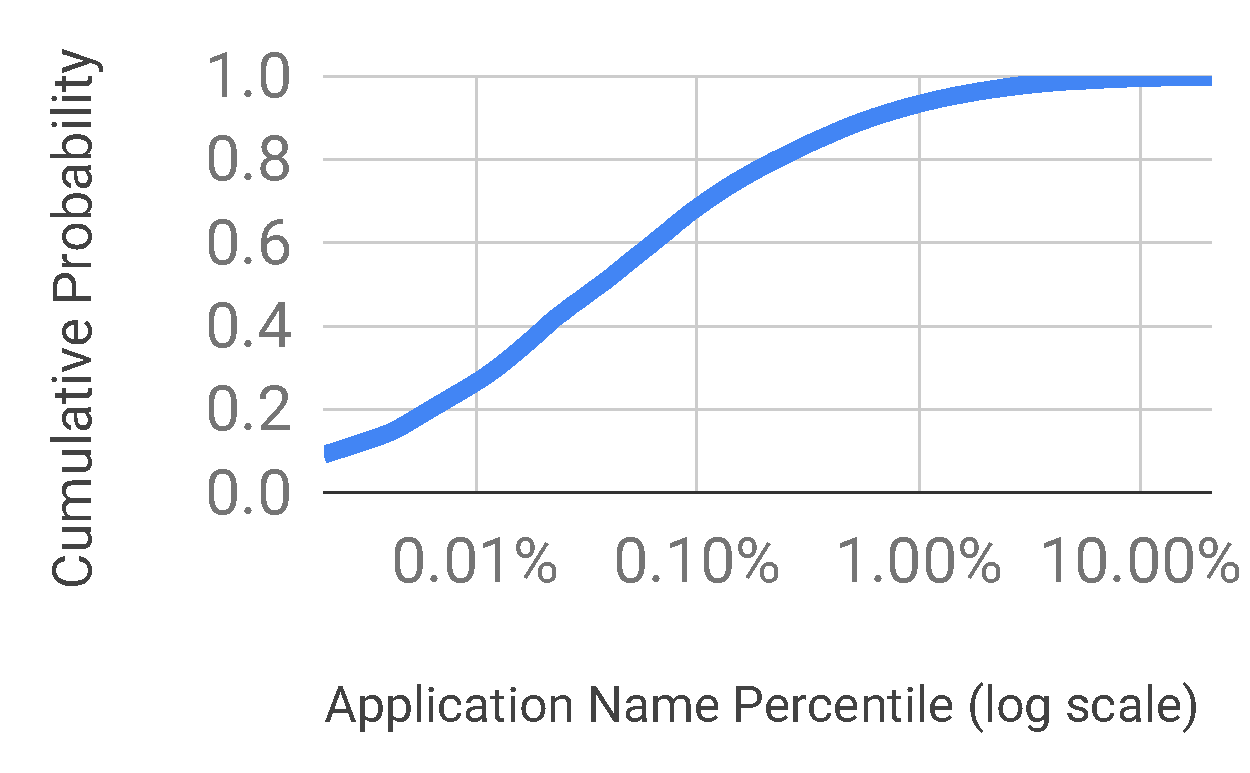
\includegraphics[width=0.8\columnwidth]{figs/cdf.pdf}
\caption{
{Application name CDF in Flurry workload.}
}
\label{fig:cdf}
%\end{wrapfigure}
\end{figure}
Figure~\ref{fig:cdf} depicts the cumulative distribution function of application name in $4$ minutes of Flurry data consisting of $200$M events of over $40$K applications.
It shows that $10$\% of the applications cover over $99.5$\% of the events; $1$\% of the applications cover $94$\% of the events; and less than $0.1$\% cover $70$\% of the events. This means the data is highly skewed and with a very long tail (not depicted in the figure).
Table~\ref {table:popular} shows the cumulative probability of the top-$20$ popular applications, covering more than $50$\% of the events. 
With application name as the primary dimension of a composite key this distribution induces high spatial locality.


\begin{table}[tb]
\center
{\footnotesize{
\begin{tabular}{|l|c|c||l|c|c|}
\hline 
  & \#events & cumulative &  & \#events & cumulative  \\
  &  &  probability& &  &  probability \\
\hline 
1 & 19,272,320 & 0.091 &11 & 4,176,189 & 0.419\\
2 & 11,424,325 & 0.146&12 & 3,109,832 & 0.434\\
3 & 11,340,475  & 0.200&13 & 3,106,912 & 0.449\\
4& 8,232,683 &0.239 &14 & 2,512,155 & 0.460\\
5& 6,579,999 &0.270 &15& 2,474,689 & 0.472\\
6& 6,172,832 & 0.299&16 & 2,343,138 & 0.483\\
7& 5,960,979 & 0.327&17 & 2,184,674 &0.494 \\
8 & 5,530,707& 0.354&18 & 1,973,152& 0.503\\
9& 4,948,991 & 0.377&19 & 1,971,366& 0.512\\
10 & 4,657,214 & 0.399&20 & 1,964,174& 0.522\\
\hline 
\end{tabular}
}}
\caption{{Top-20 popular applications cumulative probability in 4 minutes of Flurry workload.}}
\label{table:popular}
\end{table}



% Overfitting for Zipf 
The prevalence of temporal locality (i.e., frequent access to popular entities) in real-world workloads is widely-recognized.
Standard benchmarks (e.g., YCSB~\cite{YCSB})  feature skewed key-access distributions such as Zipf.
Nevertheless, 
these benchmarks fail to capture the spatial aspect of locality.
This, in turn, leads to storage systems being optimized for a skewed distribution on individual keys with no spatial locality,
e.g., by partitioning data temporally (by recent access) as opposed to by key range.
In this work, we make spatial locality a first class consideration in KV-store design.
% which leads us to rethink the design principles underlying today's popular KV-stores.

% LSM is the standard but not ideal for this  because of  write path  temporal grouping leading to fragmentation and write amplification
The de facto standard approach to building KV-stores today is \emph{LSM} (log-structured merge) trees~\cite{DBLP:journals/acta/ONeilCGO96}. 
The LSM approach optimizes write performance by absorbing random writes in memory and periodically flushing 
them as sequential files to disk. %While  sequential disk access dramatically improves I/O throughput, it 
% is important to n
Notice that the LSM design initially groups writes  into files \emph{temporally}, and not by key-range. 
A background \emph{compaction} process later merge-sorts any number of files, grouping data by keys. 
This approach is not ideal for workloads with high spatial locality for two reasons. 
First, a popular key range will be fragmented across many files during long periods (between compactions). 
Second,  compaction  is costly in terms of  both performance 
(disk bandwidth) and \emph{write amplification}, namely the number of physical writes 
associated with a single application write. The latter is  particularly important in SSDs as it increases disk wear. 
The temporal grouping means that compaction is indiscriminate with respect to key popularity:  
Since new files are always merged with old ones, 
 ``cold'' key ranges
 % that has not been accessed since the  beginning of time 
 continue to be repeatedly re-located
by  compactions.  

\remove{
% LSM is the standard but not ideal for this also in read path.
Because LSM's in-memory component consists only of recently-written keys, 
it does not contain keys that are frequently read without being modified. 
This causes \emph{read amplification}, where a read has to search for the 
requested key in multiple locations. 
In order to optimize the read-path, LSMs  use a cache of popular file blocks and 
Bloom filters that reduce unnecessary file access. 
But  a key range is typically dispersed over multiple cache blocks and Bloom filters. 
This memory organization does not leverage spatial locality, 
resulting in sub-optimal use of memory resources in case such locality is present.
Furthermore, it does not naturally lend itself to range scans,
which are common with composite keys.
}

% LSM is not the best when the entire working set fits in memory
Finally, we note that LSM's temporal  organization optimizes disk I/O but induces a penalty on in-memory operation. 
All keys -- including popular ones -- are flushed to disk periodically, even though persistence is assured 
via a separate \emph{write-ahead-log (WAL)}.
This increases write amplification and also makes the flushed keys unavailable for fast read from memory,
which is particularly wasteful if the system incorporates sufficient DRAM to hold most of the active working set. 
The drop in DRAM prices (more than $6.6$x since 2010~\cite{dram-prices})  
%and significant performance benefit DRAM offers 
makes this scenario increasingly common.  

%\subsection{\sys} 
The main goal of this work is to propose a design alternative  that is better suited for spatial locality workloads. 

% Drum roll 
We present \sys, a persistent KV-store whose design diverges from the ubiquitous LSM approach.  
Like  LSMs,  we optimize I/O by absorbing updates in memory before writing to disk. 
But unlike LSM's temporal data organization, we partition data by key, as in B-trees~\cite{Comer79} and B$^\epsilon$-trees~\cite{Bender15}. 
Data is  organized (both on disk and in memory) as a list (rather than a tree) 
of large \emph{chunks} holding contiguous key ranges.
To allow direct access (one I/O operation) to the on-disk chunk holding a given key, we use an auxiliary volatile index.  
In addition, popular chunks are cached in RAM for the benefit of  both the write-path and the read-path.
% and as in LSM, popular keys are cached for read access.

% Benefits
Spatially-organized chunks reduce the fragmentation of key ranges, resulting in 
(1) better read and write performance for workloads with spatial locality,  and
(2) faster range scans. 
Moreover, since chunks  are compacted in memory, writes are 
flushed to disk less frequently than LSM writes (relying on a per-chunk WAL for persistence)
yielding 
(3) reduced write amplification, and 
(4) better performance when most of the working set fits in memory.

% Downsides
The downside of this approach is that if the data lacks spatial locality and the active working set is big, 
caching an entire chunk for a single popular key is wasteful. We mitigate this  by adding 
a dedicated \emph{row cache} for hot keys. 
%But since the row cache only serves the read-path, 
%this design is less optimal for mixed read/write workloads lacking spatial locality,
%where the LSM approach may be more suitable.  

\sys's APIs (put, get, and scan) provide strong consistency guarantees 
under concurrency.  Its performance scales with the number of threads on multicore hardware, 
and
% We employ scalable concurrent data structures for in-memory processing. %, to scale with the number of cores. 
in addition, \sys\/ recovers from crashes quickly since it does not need to replay the WAL on recovery.

We implemented \sys\ in C++. 
We compare it to the recent release of RocksDB~\cite{RocksDB}, 
an industry-leading LSM KV-store.
Our experiments, based on Flurry data show ingestion throughput is up to 3.8x higher for \sys, while write amplification is 2.4x-4x higher for RocksDB. \sys improves short scans speed by 90\% in medium size data bases and by 20\%-50\% in long scans and large databases.
%, as well as to PebblesDB~\cite{PebblesDB}, a research LSM store with low write amplification. 

Experiments based on the popular YCSB benchmark suite~\cite{YCSB}, 
show \sys\/ significantly outperforms RocksDB when spatial  locality is high, and also 
whenever most of the working set fits in RAM. For example, with composite keys and a memory-resident 
working set, \sys\  accelerates scans by up to $2$x, puts by up to $2.3$x, and gets by up to $2$x. 
With larger working sets, \sys\ still improves over RocksDB's throughput by $24\% - 75\%$. In traditional
YCSB workloads,  \sys\ is comparable to RocksDB. RocksDB performs better than 
\sys\ in mixed read/write workloads with large active working sets and no spatial locality. 
%(2) \sys\/ outperforms PebblesDB by a wide margin under all workloads, especially in high-concurrency 
%scenarios (up to $2.9$x in puts, $3.2$x in gets, and $4.5$x in scans). 

%As with all new approaches, there is ample  room for future improvements. 
  % The rest of this paper is organized as follows ... 
\remove{
We present our design principles in~\cref{sec:principles} and  the \sys\ algorithm 
in~\cref{sec:design}. We then discuss implementation details in~\cref{sec:impl} and evaluate 
\sys\ in~\cref{sec:eval}.  Finally,~\cref{sec:related}   surveys related work and~\cref{sec:conclusions}
concludes.
} 
